\chapter{轨迹与作图}
在前面的几章中,我们学习了直线形和圆的有关性质。
学习的途径主要是根据图形的定义和已知性质去推演图形的
其它性质。这一章,我们将把图形看成点的集合(点集),
研究如何根据点所具有的某种性质来求出点集在平面上的形
状和位置。

\section{轨迹}
\subsection{轨迹的概念}
我们知道,物体在运动中都要经过一定的路线。例如,
人在雪地里行走会留下明显的足迹,飞机飞行有一定的航
线,地球运行也有它的轨道等等。一般,我们常把物体按某
种规律运动的路线叫做物体运动的\textbf{轨迹}。在几何中,我们用
点表示物体在空间的位置。这样,一个点在空间按某种规律
运动的路线,我们就把它叫做这个点运动的轨迹,这个点就
叫做\textbf{动点}。例如,我们用圆规画圆时,圆规的一个脚尖固定
不动,而另一个脚上装上的铅笔尖端就可看作一个动点。它
和固定的脚尖保持一定的距离运动,所画出的图形就是这个
动点的轨迹。我们知道,圆是“同一平面上和某定点的距离
等于定长的点的集合”。由此可见,按某种规律运动的点的
轨迹,也就是具有某种性质的点的集合。

\begin{blk}{定义}
具有性质$\alpha$的所有点构成的集合,叫做具有性
质$\alpha$的点的轨迹。
\end{blk}

设$X=\{\text{具有性质$\alpha$的点}\}$。由上述定义,当我们要证明
某图形$A$是具有某种性质$\alpha$的点的轨迹时,也就是要证明
集合$A=X$. 要证明$A=X$, 就必须从以下两方面进行证
明:
\begin{enumerate}
\item $P$点$\in A\Rightarrow P$点具有性质$\alpha$ $(P\in X)$.
\item $P$点具有性质$\alpha$ $(P\in X)\Rightarrow P$点$\in A$.
\end{enumerate}

按上述两个方面证明,这是缺一不可的。如果我们只证
了第一条,实际上只是说明$A$是$X$的一个子集,并不能断
定$A=X$; 如果只证了第二条,也只是说$X$是$A$的一个子
集,同样不能断定$A=X$, 只有当我们证明了第一条:$A\subseteq
X$, 又证明了第二条:$X\subseteq A$, 我们才能断定$A=X$.

第一条证明了$A\subseteq X$, 这就是说在图形$A$上的点,都具
有性质$\alpha$. 没有一点是鱼目混珠的,通常把证这一条叫做证
\textbf{轨迹的纯粹性}。第二条证明了$X\subseteq A$, 这就是说,具有性质
$\alpha$的点都在图形$A$上,没有一点被遗漏掉。通常又把证这一
条叫做证\textbf{轨迹的完备性}。

由于原命题与逆否命题等价,所以也可以分别去证上述
两条的逆否命题,即要证轨迹的纯粹性也可证:
\[P\text{点不具有性质}\alpha\Rightarrow P\notin A\]
要证轨迹的完备性时,也可证:
\[P\text{点}\notin A\Rightarrow P\text{点不具有性质}\alpha\]

\begin{ex}
\begin{enumerate}
\item 叙
述两个集合相等的定义。
\item 在证轨迹命题时,为什么即要证轨迹的纯粹性,又要证
轨迹的完备性?
\item 如果我们证明了
$\overline{AB}$的垂直平分线上的任一点到$A$、
$B$两
点的距离相等,能否就说与$A$、$B$两点距离相等的点
的轨迹是$\overline{AB}$的垂直平分线?
\end{enumerate}
\end{ex}


\subsection{基本轨迹}
这一小节,我们来学习六个平面上的点的基本轨迹,我
们只证了1和4, 其它四个由同学们自证。

\begin{blk}{基本轨迹1}
与两个已知点距离相等的点的轨迹是连结
这两点的线段的垂直平分线。
\end{blk}

已知:两定点$A$、$B$, 直线$MN$是$\overline{AB}$的垂直平分线(图5.1)。

求证:与$A$、$B$两点距离相等的点的轨迹是直线$MN$.

\begin{figure}[htp]
    \centering
\begin{tikzpicture}[scale=.7]
\draw(-2,0)node[left]{$A$}--(2,0)node[right]{$B$};
\draw (0,3)node[above]{$M$}--(0,-2.5)node[below]{$N$};
\draw[dashed](-2,0)--(0,2.5)node[left]{$P$}--(2,0)--(0,-1.8)node[left]{$Q$}--(-2,0);
\node at (.25,.25){$O$};

\end{tikzpicture}
    \caption{}
\end{figure}


\begin{proof}
\begin{enumerate}
    \item 
设$P$是直线$MN$上的任一点,作$\overline{PA}$、$\overline{PB}$,
在$\triangle AOP$与$\triangle BOP$中,

$\because\quad \overline{AO}=\overline{BO},\quad \angle AOP=\angle BOP,\quad \overline{OP}=\overline{OP}$

$\therefore\quad \triangle AOP\cong \triangle BOP$ (SAS),
$\overline{PA}=\overline{PB}$.

这就说明了直线$MN$上的点,都与两点的距离相等。

\item 设$Q$为与$A$、$B$等距的点,即$\overline{QA}=\overline{QB}$. 过$AB$的
中点$O$与$Q$作直线$OQ$, 根据等腰三角形的性质,直线$OQ$
垂直平分$\overline{AB}$, 但$\overline{AB}$的垂直平分线只有一条,

$\therefore\quad MN$与$OQ$重合,$Q\in MN$.

\end{enumerate}

于是由1、2可知,与$A$、$B$两点距离相等的点的
轨迹是直线$MN$.
\end{proof}

\begin{blk}
{基本轨迹2} 与已知角的两边距离相等的点的轨迹是这
个已知角的平分线。
\end{blk}

\begin{blk}
{基本轨迹3} 与两条平行线等距离的点的轨迹是和这两
条平行线平行且平分它们的公垂线段的直线。
\end{blk}

\begin{blk}
    {基本轨迹4}与一条直线的距离等于定长的点的轨迹,是
    平行于这条直线,并和这条直线的距离等于定长的两条直线。
\end{blk}

已知:直线$CD\parallel$直线$AB$; 直线$EF\parallel$直线$AB$; $CD$、$EF$和$AB$之间的距离都是$d$(图5.2)。

求证:与$AB$的距离等于
$d$的点的轨迹是$CD$和$EF$.

\begin{figure}[htp]
    \centering
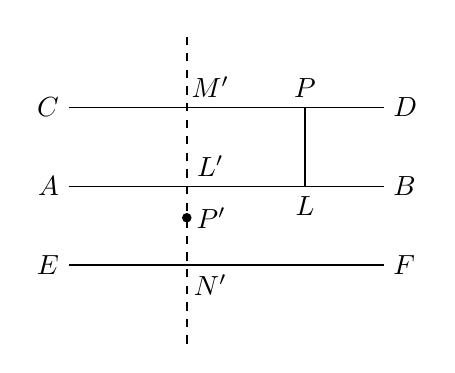
\begin{tikzpicture}
\draw (0,0)node[left]{$E$}--(4,0)node[right]{$F$};
\draw (0,1)node[left]{$A$}--(4,1)node[right]{$B$};
\draw (0,2)node[left]{$C$}--(4,2)node[right]{$D$};
\draw[dashed, thick] (1.5,-1)--(1.5,3);
\draw[thick] (3,1)node[below]{$L$}--(3,2)node[above]{$P$};
\node at (1.8,0)[below]{$N'$};
\node at (1.8,1)[above]{$L'$};
\node at (1.8,2)[above]{$M'$};
\draw (1.5,.6) [fill=black] circle (1.5pt) node[right]{$P'$};
\end{tikzpicture}
    
    \caption{}
\end{figure}


\begin{proof}
\begin{enumerate}
    \item 设$P$是$CD$或$EF$ 上的任一点。作$PL\bot AB$于$L$点。

$\because\quad CD\parallel AB$且和$AB$的距离等于$d$

$\therefore\quad \overline{PL}$是$AB$和$CD$的公垂线段,且$\overline{PL}=d$.

这就是说$CD$上的任一点和$AB$的距离都等于$d$, 同理
可证$EF$上的任一点和$AB$的距离也都等于$d$.
\item 设$P'$点是不在$CD$或$EF$上的任一点。
经过$P'$点作垂直于$AB$的直线,分别交$AB$、$CD$、$EF$于
$L'$、$M'$、$N'$, 则$\overline{M'L'}=\overline{N'L'}=d$.

$\because\quad P'$不在$CD$或$EF$上

$\therefore\quad P'$不和$M'$、$N'$重合

$\because\quad $在直线$M'N'$上和$L'$距离等于$d$的点只有$M'$、$N'$

$\therefore\quad \overline{P'L'}\ne d$

这就是说,不在$CD$和$EF$上的任何一点和$AB$的距离都
不等于$d$.
\end{enumerate}

于是由1、2可知,和$AB$的距离等于$d$的点的轨
迹是$CD$和$EF$。
\end{proof}

\begin{blk}
    {基本轨迹5} 与一个定点的距离等于定长的点的轨迹,
是以定点为圆心,定长为半径的一个圆。
\end{blk}

\begin{blk}
    {基本轨迹6}与一条定线段的两端连线所夹的角等于定角的点的轨迹,是以这条定线段为弦,所含的圆周角等于定
    角的两条弧。
\end{blk}

以上六个基本轨迹是研究其它轨迹问题的基础,同学们
一定要熟记。

\begin{example}
    求已知圆内等于定长的弦的中点的轨迹。

    已知$\odot (O,r)$和定长$a$, 且$a<2r$(图5.3)。

    求$\odot (O,r)$内等于定长$a$的弦的中点的轨迹。
\end{example}

\begin{figure}[htp]
    \centering
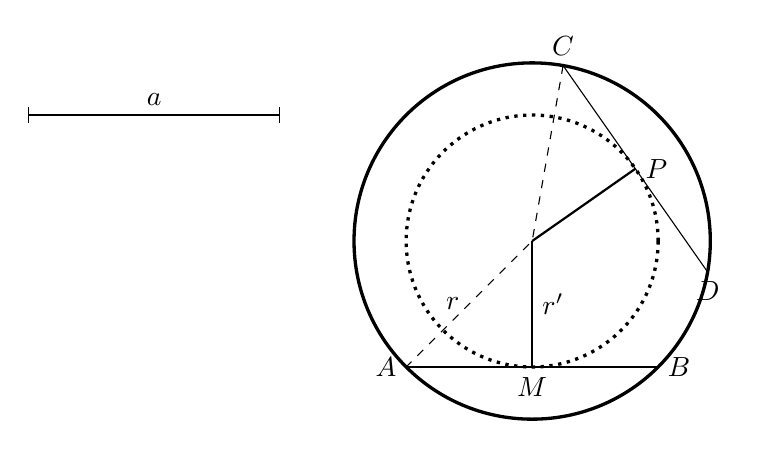
\begin{tikzpicture}[scale=1.6]
\draw[very thick] (0,0) circle (1.414)  ;  
\draw[very thick, dotted] (0,0) circle (1)  ;  
\draw (-45:1.414)node[right]{$B$}--(-45-90:1.414)node[left]{$A$};
\draw[dashed] (80:1.414)--(0,0)--node[left]{$r$}(-45-90:1.414);
\draw [thick] (0,0)--node[right]{$r'$}(0,-1)node[below]{$M$};
\draw (80:1.414)node[above]{$C$}--(-10:1.414)node[below]{$D$};
\draw [thick] (0,0)--(35:1)node[right]{$P$};

\draw[|-|](-4,1)--node[above]{$a$}(-2,1);
\end{tikzpicture}
    \caption{}
\end{figure}

\begin{solution}
    如图5.3, 设$\overline{AB}$是$\odot (O,r)$内等于定长$a$的弦,$M$
是它的中点,作$\overline{OM}$, 那么,$\overline{OM}\bot \overline{AB}$。
\[\overline{AM}=\frac{1}{2}\overline{AB}=\frac{a}{2}\]
所以
\[\overline{OM}=\sqrt{\overline{OA}^2-\overline{AM}^2}=\sqrt{r^2-\left(\frac{a}{2}\right)^2}\]
设$r'=\sqrt{r^2-\left(\frac{a}{2}\right)^2}$,则$r'$
为定长,以$O$为圆心,$r$为
半径画$\odot (O,r')$, 那么,$\odot (O,r)$内等于定长$a$的弦的中
点都在$\odot (O,r')$上。另外,在$\odot (O,r')$上任取一点$P$, 作
$\overline{OP}$, 再作弦$\overline{CD}\bot\overline{OP}$于$P$点,则$P$点是$\overline{CD}$弦的中点,且
\[\overline{CD}=2\overline{CP}=2\sqrt{r^2-{r'}^2}=2\sqrt{r^2-\left[r^2-\left(\frac{a}{2}\right)^2\right]}=2\cdot\frac{a}{2}=a\]
这就是说$\odot (O,r')$上的任一点都是$\odot (O,r')$内等于定长$a$
的一条弦的中点,所以我们所求的轨迹就是$\odot (O,r')$。
\end{solution}

\begin{example}
    过定圆外一定点引圆的割线,求割线被圆截下的弦的中点的轨迹。

    已知:定$\odot (O,r)$和$\odot O$外定点$P$(图5.4)。
    
    求:过$P$点引$\odot O$的割线,被$\odot O$截下的弦的中点
    的轨迹。
\end{example}


\begin{figure}[htp]
    \centering
\begin{tikzpicture}[scale=1.2]
\tkzDefPoints{0/0/O, 2.5/0/O', 5/0/P}
\draw[dashed] (P)--(-2,0)node[left]{$E'$};
\draw (0,0) circle (2);
\draw[dashed] (O') circle (2.5);
\tkzDefTangent[from with R=P](O, 2cm)
\tkzGetPoints{A}{B}
\tkzDrawSegments[add=0 and .2](P,A  P,B)
\node at (-.25,-.25){$O$};\node at (.25+2.5,.25){$O'$};
\node at (2.2,0)[above]{$E$};
\tkzDrawPoints(O',O)
\tkzDefShiftPoint[O'](150:2.5){M}
\tkzDefShiftPoint[O'](-142:2.5){N}
\tkzDefShiftPoint[O'](-155:2.5){X}
\tkzAutoLabelPoints[center=O'](M,N,X,A,B,P)
\tkzInterLC(P,M)(O,A) \tkzGetPoints{C'}{C}
\tkzInterLC(P,X)(O,A)\tkzGetPoints{D}{D'}
\tkzInterLC(P,N)(O,A)\tkzGetPoints{F}{F'}
\tkzAutoLabelPoints[center=O](D,F,C,C',D',F')
\draw(C')--(P)--(F');
\draw(D')--(P);
\draw[dashed](M)--(O)--(X);
\draw[dashed](A)--(O);
\end{tikzpicture}
    \caption{}
\end{figure}

\begin{solution}
    由于轨迹是具有某种性质$\alpha$的点的集合,求轨迹时,可先按照“性质”画出一些点,看看这些点可
能构成什么样的图形,如图
5.4, 过$P$点作$\odot O$的割线,与$\odot O$相交于$C$、$C'$, 作弦
$\overline{CC'}$的中点$M$, 我们证割线$PCC'$绕$P$点旋转,看这条变动
的割线被$\odot O$截下的弦的中点经过什么路线。大概可以看
出,可能是一段圆弧,究竟是不是圆弧,如果是圆弧,又如
何把它作出来,还要进一步分析。

$\because\quad M$是弦$\overline{CC'}$的中点,作$\overline{OM}$

则$\overline{OM}\bot\overline{CC'}$,即:$\angle OMP$是直角。

这就是说,过$P$点作$\odot O$的任一条 割线
被$\odot O$截下的弦的中点与$O$、$P$的连线的夹角等于直角,因
此,符合题中条件的弦的中点都在以$\overline{OP}$
为直径的圆上,以$\overline{OP}$
为直径作$\odot O'$, 我们所作的$\odot O'$是不是就是所求的轨迹呢?
这还要看$\odot O'$上有没有不符合条件的点。设$\odot O'$与$\odot O$相
交于$A$、$B$两点。显然,在$\odot O'$上$\wideparen{AOB}$外的点都是不合条
件的(包括$A$、$B$),我们再来看$\wideparen{AOB}$上的点是不是都是合
条件的点。在
$\wideparen{AOB}$上任取一点$X$, 设$PX$与$\odot O$相交于$D$、
$D'$, 作$\overline{OX}$, 则$\overline{OX}\bot \overline{DD'}$,所以$X$是$\overline{DD'}$的中点,这就
是说$\wideparen{AOB}$上的点都是过$P$点的某条割线被$\odot O$截下的弦的中
点。
\end{solution}

综合以上分析我们可得:过定圆外一定点引圆的割线,
割线被圆截下的弦的中点的轨迹是以定点与圆心间的线段为
直径的圆被夹在定圆内的一段弧。

\begin{ex}
    说出下列的点的轨迹是什么图形?并把它们分别画出
来。
\begin{enumerate}
    \item 到一条5cm长的线段的两端距离相等的点的轨迹。
    \item 通过两定点的圆的圆心的轨迹。
    \item 到一个等于60$^{\circ}$的已知角的两边距离相等的点的轨述:
    \item 与两条相交直线等距离的点的轨迹。
    \item 与$\angle AOB$的两边都相切的圆的圆心的轨迹。
    \item 与距离是3cm的两条平行直线$AB$、$CD$的距离相等的点
的轨迹。
\item 与距离是3cm的两条平行直线都相切的圆的圆心的轨
迹。
\item 和已知直线$AB$的距离等于2cm的点的轨迹。
\item 和已知直线$AB$相切,并且半径等于1.5cm的圆的圆心
的轨迹。
   \item 和一条已知直线切于已知点的圆的圆心的轨迹。
\item 与定点$A$的距离等于2cm的点的轨迹。
\item 和一条长是3cm的$AB$的两端连线所夹的角是直角的点
的轨迹。
\item 和一条长是4cm的已知线段$AB$的两端连线所夹的角等
于60$^{\circ}$的点的轨迹。

\end{enumerate}
\end{ex}


\section*{习题5.1}
\addcontentsline{toc}{subsection}{习题5.1}
\begin{enumerate}
    \item 求下列轨迹
\begin{enumerate}
    \item 以已知$\overline{AB}$为一边的三角形的外心的轨迹。
    \item 以已知$\overline{AB}$为一边,并且这边上的中线的长等于定长$m$的三角形的重心的轨迹。
\item 以3cm长的已知$\overline{AB}$为一边,并且面积等于6平方厘
米的三角形的顶点$C$的轨迹。
\item 和一个半径等于定长$r$的$\odot O$外切,并且半径等于
$r'$的圆的圆心的轨迹。
\item 以已知$\overline{BC}$为斜边的直角$\triangle ABC$的顶点$A$的轨迹。
\end{enumerate}

\item 叙述符合下列条件的点的轨迹。
\begin{enumerate}
    \item 平行于三角形的一边而夹在其余两边之间的线段的
中点的轨迹。
\item 平行于已知直线而在已知圆内的弦的中点的轨迹。
\end{enumerate}
\item 作出下列各题中给出的两个点集,向它们的交集各含有
几个元素。

\begin{enumerate}
    \item 和距离等于3cm的两条已知平行线$AB$、$CD$的距离
相等的点集;和直线$AB$上的一定点$E$的距离是2cm的点
集。
\item 和已知$\angle AOB$的两边的距离相等的点集;和边$OA$
的距离等于$d$的点集。
\item 和一条长3cm的已知$\overline{AB}$的两端连线所夹的角是直角
的点集;和$\overline{AB}$所在直线距离等于2cm的点集。
\end{enumerate}


\item 求通过$\odot (O,r)$内一定点$P$的弦的中点的轨迹。
\item 求到$\odot(O,3{\rm cm})$的圆面等于4cm的点的轨迹。
\end{enumerate}

\section{作图}
\subsection{基本作图}
在前几章中,我们曾用直尺、圆规解过不少作图题。在
这一节里,我们将进一步学习解作图题的一些重要方法,下
面列出我们已经学过的一些作图题(具体作法不再写出,由
同学自己复习、研究),这些作图题一般叫做\textbf{基本作图题},
它们是进一步解较复杂的作图题的基础。
\begin{enumerate}
\item 作一条线段等于已知线段,作一条线段等于$n$条线
段的和($n\ge 2$ 且 $n\in\mathbb{N}^+$)。
\item 作一条线段等于两条已知线段的差。
\item 作一个角等于已知角。
\item 平分一个已知角。
\item 过已知直线上或已知直线外一点,作已知直线的垂
线。
\item 作已知线段的垂直平分线。
\item 等分已知线段。
\item 按已知条件作三角形。
\begin{enumerate}
 \item 已知三边。
\item 已知两边及其夹角。
\item 已知两角及其中一角的对边。
\item 已知两角及其夹边。 
\end{enumerate}
\item 作三角形的外接圆和内切圆。
\item 已知斜边和一直角边,作直角三角形。
\item 已知线段$a$, 作一线段$x=\frac{m}{n}a$. (其中$\frac{m}{n}$
是正有理数)。
\item 作已知三条线段$a$、$b$、$c$的比例第四项。
\item 已知线段$a$、$b$, 作$a$、$b$的比例中项。
\item 已知线段$a$、$b$ $(a>b)$, 作线段$x=\sqrt{a^2+b^2}$
或$x=\sqrt{a^2-b^2}$。
\item 已知线段$a$, 作线段$x=\sqrt{\frac{m}{n}}a$ ($\frac{m}{n}$为正有理数)。
\item 过已知圆上一点作圆的切线。
\item 过已知圆外一点作圆的切线。
\item 作两个已知圆的公切线。
\item 过已知直线外的一个已知点,作这条直线的平行
线。
\end{enumerate}

\begin{ex}
\begin{enumerate}
    \item 作一直角三角形$ABC$, 使$\angle C=90^{\circ}$, $AB=3$cm, $BC=
    2$cm. 你能想出几种作法?
    \item 已知线段$a$、$b$,你能用几种方法作线段$x=\sqrt{ab}$。
    \item 已知线段$a$, 作线段$x=\sqrt{\frac{2}{3}a}$
        \item 过圆外一点,你能用几种方法作这个圆的切线。
\end{enumerate}
\end{ex}

\subsection{轨迹法作图}
我们在解作图题时,常常归结为要确定某些点的位置,
而这些点所要满足的条件又往往不是一个,我们只要根据点
所满足的各个条件,分别作出相应的轨迹,那么,这些轨迹
交集中的点,就是我们所要求作的点。

例如,已知两个定点$B$、$C$, 且
$\overline{BC}=3$cm (图5.5),以
$B$、$C$为两个顶点,求作一三角形,使第三个顶点与$B$的距
离是2cm, 与$C$的距离是4cm, 这个作图题,实际上就是确定
三角形的第三个顶点的位置。第三个顶点要满足两个条件:
\begin{enumerate}
    \item 和$B$点的距离是2cm
    \item 和$C$点的距离是4cm
\end{enumerate}
满足第一个条件的点的轨迹是$\odot(B,2{\rm cm})$,满足第二个条件的
点的轨迹是$\odot (C,4{\rm cm})$,所以第三个顶点就应该是$\odot(B,2{\rm cm})$与$\odot (C,4{\rm cm})$的交集中的点。由作图可知:
\[\odot(B,2{\rm cm})\cap \odot (C,4{\rm cm})=\{A, A'\}\]
于是,$A$点和$A'$点都是我们所
要求作的点,$\triangle ABC$与$\triangle A'BC$都是我们所要求作的三角
形。像这样应用轨迹的交集来确定点的位置,从而来解作图
题的方法,就叫做\textbf{轨迹法}。


% P86






































































